\documentclass[12pt,a4paper]{scrartcl}
\usepackage[utf8]{inputenc}
\usepackage[german]{babel}
\usepackage[T1]{fontenc}
\usepackage{amsmath}
\usepackage{graphicx}
\usepackage{caption}
\usepackage{float}
\usepackage{subcaption}

\title{Evolutionärer Algorithmus -- EvoTest}
\author{Yaroslax, Alexander, Manuel}

\begin{document}
\section{Genetischer Algorithmus}
Der genetische Algorithmus dient zur iterativen Optimierung der Testfälle. Er erzeugt eine Anzahl Chromosome, die über mehrere Stufen durch diverse Operationen verbessert werden.

\subsection{Architektur}
% Alex, evntl UML, umsetzung, etc
Der Genetische Algorithmus wird als eine Klasse implementiert (s. Abbildung \ref{fig:ga_uml}).\\
In der Mutation- und ReproductionRate wird festgelegt, wie stark ein Chromosom mutieren soll oder wie viele neue Chromosome der Population pro Epoche hinzugefügt werden, bevor die Population wieder auf Soll-Größe schrumpft.\\
Da die Implementierung der einzelnen Schritte auf Modularität ausgelegt ist (s. Absatz \ref{sec:op}), werden einige der Funktionen als Eigenschaften gesehen, da sie modular austauschbar sind.\\
Die Ausführung des Genetischen Algorithmus findet in der main Methode statt (s. Abbildung \ref{fig:ga_flow}). Diese akzeptiert unter Umständen noch Parameter, welche zur Berechnung des Abbruchkriteriums genutzt werden. Aktuell bricht der genetische Algorithmus stets nach einer übergebenen Anzahl Epochen ab. Dies kann aber angepasst werden, falls es im weiteren Verlauf des Praktikums noch vonnöten wäre.
\begin{figure}[H]
\centering
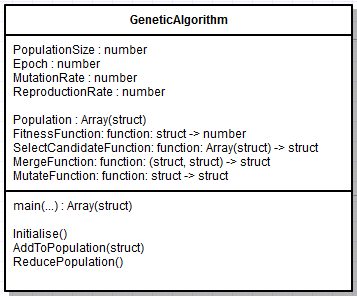
\includegraphics[width=.5\textwidth]{images/GA_UML}%
\caption{Klassenkarte des Genetischen Algorithmus}%
\label{fig:ga_uml}%
\end{figure}

\begin{figure}[H]
\centering
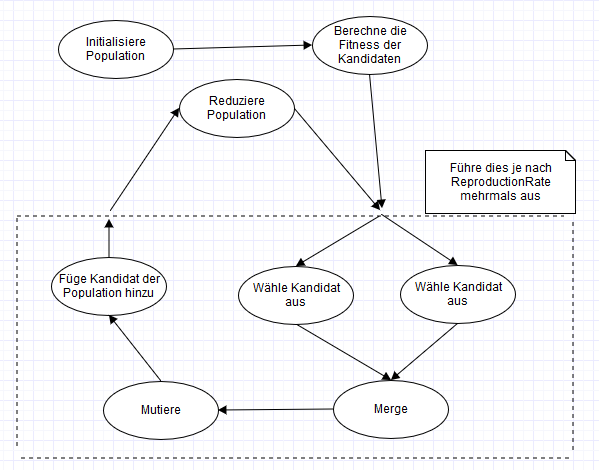
\includegraphics[width=.75\textwidth]{images/GA_FlowChart}
\caption{Ablauf des genetischen Algorithmus}
\label{fig:ga_flow}
\end{figure}

\subsection{Chromosome}
% Parameterisierung (Prozent der Range)
% Manuel
Chromosome dienen der Persistierung der Testfall-Konfigurationen. Sie enthalten die Bestandteile eines realen Testfalls -- so wie er für die Simulation benutzt wird -- in einer für den Genetischen Algorithmus geeigneten Kodierung. Abbildung \ref{fig:chromosome} bietet einen Überblick über die Bestandteile.
\begin{figure}[H]
\centering
\begin{tabular}{|l|}
\hline
Chromosome\\
\hline
carx \\
cary\\
carangle\\
slotlength\\
slotdepth\\
\hline
\end{tabular}
\caption{Bestandteile eines Chromosoms}
\label{fig:chromosome}
\end{figure}
Die Information in den Chromosomen sind als prozentualer Anteil eines Wertebereichs kodiert. Die Unterteilung der Wertebereiche erfolgt durch eine 8-Bit Diskretisierung, somit entsprechen 0\% dem Wert 0 und 100\% dem Wert 255. Tabelle \ref{tab:ranges} stellt die tatsächliche Verteilung der Werte dar. 
\begin{table}[H]
\centering
\begin{tabular}{l|c|c}
Wert & Minimum & Maximum \\\hline
Fahrzeug X-Koordinate & -7.5 & +7.5 \\
Fahrzeug Y-Koordinate & -1 & +4 \\
Fahrzeug Orientierung & 0 & $2\,\pi$\\
Slot-Länge & 2.25 & 5 \\
Slot-Breite & 1 & 2 \\
\end{tabular}
\caption{Wertebereiche der Chromosom-Bestandteile}
\label{tab:ranges}
\end{table}
Die Chromosomen werden in Matlab in einer eigenen Klasse abgelegt. Sie speichert die zugewiesenen prozentualen Anteile an der Gesamt-Range sowie die zugeordnete Fitness. Zudem wird eine Funktion angeboten, die die Berechnung des durch das Chromosom repräsentierten Szenarios -- und somit das Mapping auf die spezifizierten Wertebereiche -- vornimmt.


\subsection{Austauschbare Operatoren}\label{sec:op}
% Faktory-Pattern, Einbindung in gen GA
% Manuel, Alex
Um eine skalierende Lösung vorzuhalten -- insbesondere im Hinblick auf Erweiterungen und Optimierungen -- wurden die Teil-Implementierungen des Evolutionsprozesses austauschbar realisiert. Sie werden als \emph{Function-Handle} im Evolutionsframework verankert und können zu Beginn oder nach einer gewissen Epoche durch eine Funktion mit äquivalenter Signatur getauscht werden. So ist es Beispielsweise möglich, Anfangs nach vielversprechenden Bereichen zu suchen, um im späteren Verlauf eine lokale Optimierung durchzuführen.

\paragraph{Operatoren Erzeugung} Die Operatoren werden durch das \emph{Factory-Pattern} generiert. Dabei wird eine Fabrik-Funktion verwendet um die Operation gegebenenfalls zu konditionieren. Sie liefert als Resultat die fertige Operation, die in den genetischen Algorithmus eingebunden werden kann.

\section{Operatoren}
Die Operatoren, die im genetischen Algorithmus angewendet werden, sind modular tauschbar. Sie müssen lediglich die Schnittstellendefinition einhalten.

% BEGIN Init
\subsection{Initialisierung}
\paragraph{Erklärung}
Die Initialisierung erzeugt die initiale Population aus N Chromosomen für den Start vom genetischen Algorithmus. Für die Erzeugung der Population werden N Chromosome mit zufälligen Werten der notwendigen Bestandteile (carx, carx, carangle, slotdepth, slotlength) erzeugt. 

\paragraph{Implementierung}
Die Initialisierung wird in der Methode Init der Klasse GeneticAlgorithm implementiert. Es wird ein temporäres Array der Objekte der Klasse Chromosom  mit Größe N erstellt und in N Schleifendurchläufen befüllt. Je Iteration wird für jedes Bestandteil eines Chromosoms ein zufälliger Integerwert aus einer Uniformverteilung im Bereich [0, 255] generiert. Diese Werte werden folglich an den Kromosomkonstruktor übergeben. Das Ergebnis vom Konstruktor mit dem Objekt wird ins temporäre Array gespeichert. Nachdem das Array mit N Werten befüllt wurde, wird es der Eigenschaft Population des GeneticAlgorithm-Objekts zugewiesen.
\paragraph{Probleme}
Die Erzeugung eines Chromosoms mit voneinander unabhängig generierten Werten für dessen Bestandteile kann dazu führen, dass manche Chromosome für die Simulation nicht brauchbar ist. Allerdings  würden solche Chromosome im ersten Durchlauf nach Auswertung der Fitnessfunktion vom genetischen Algorithmus verworfen werden.
% END Init

% BEGIN Selektion
\subsection{Selektion}
\paragraph{Erklärung}
Die Selektion wählt die Chromosome aus der aktuellen Population aus, aus welchen man neue Chromosome generieren wird. Auch hier wird Modularität ermöglicht, obwohl es einen Standardansatz gibt. Die Schnittstelle hierfür ist folgendermaßen definiert:
\begin{quote}
 \textsf{Select: array(chromosom) $\rightarrow$ chromosome}
\end{quote}
\begin{enumerate}
	\item Die effizienteste und in vielen Fällen sogar ausreichende Selektionsfunktion wählt mit gleichverteilter Wahrscheinlichkeit ein Chromosom $x$ aus der Population $ppl$ aus $$p(x) ~=~ \frac{1}{|ppl|}$$ wobei $|ppl|$ die Menge an Elementen der Population ist.
	\item Die dem Standard entsprechende Funktion wählt ein Chromosom $x$ der Population $ppl$ mit Wahrscheinlichkeit $$p(x)~=~\frac{Fitness(x)}{\sum_{c ~\in~ ppl}^{}{Fitness(c)}}$$
\end{enumerate}
% END Selektion

% BEGIN Rekombination
\subsection{Rekombination}
\paragraph{Erklärung}
Die Rekombination führt den Crossover Teil des Genetischen Algorithmus aus. Er erstellt ein neues Chromosom wobei er für jeden einzelnen Wert entscheidet, welchem der gegebenen zwei Chromosome er diesen Wert entnimmt.\\
Die Schnittstelle für die Rekombination ist folgendermaßen definiert: 
\begin{quote}
	\textsf{merge: (chromosome, chromosome) $\rightarrow$ chromosome}
\end{quote}
\paragraph{Probleme} Die Rekombination wählt jeden Wert unabhängig von der Wahl der anderen Werte aus. Daraus kann sich das Szenario ergeben, dass die X-Position des neuen Chromosoms nicht vom gleichen Chromosom kommt, wie die Y-Koordinate. Hieraus folgt dasselbe Problem wie bei der Mutation, dass semantisch ähnliche Variablen vollständig unabhängig voneinander gesetzt werden. Auch hierfür kann man bei Bedarf die Modularität des Systems ausnutzen und eine erweiterte Crossover Funktion erstellen. Zur Zeit erweist sich die hier gewählte Funkion aber als den Anforderungen genügend.
% END Rekombination

% BEGIN Mutation
\subsection{Mutation}
% Manuel
\paragraph{Erklärung}
Die Mutation genügt der Signatur
\begin{quote}
 \textsf{mutate: chromosome $\rightarrow$ chromosome}
\end{quote}
Durch die generische Auslegung der Mutation im Rahmen des genetischen Algorithmus ist ein Austausch jederzeit möglich. Für den aktuellen Stand wurde ein Algorithmus entwickelt, der das Genom als Integer interpretiert und in dessen Binärdarstellung -- als String -- umwandelt. Dieser String wird iterativ verarbeitet. Dabei wird jedes Bit mit einer zuvor definierten Wahrscheinlichkeit umgekehrt.
\paragraph{Probleme} Die Mutation erfolgt mit einer identischen Wahrscheinlichkeit für hoch- und niederwertige Bits. Dies kann von Vorteil sein, um randomisiert auch große Sprünge zu erlauben. Allerdings können somit auch vielversprechende Kandidaten stark verändert werden. Es kann also eventuell Notwendig sein, Spezialformen der Bit-Mutation zu integrieren. Das modulare System bietet hierfür hervorragende Skalierungsmöglichkeiten.
% END Mutation

% BEGIN Fitness
\subsection{Fitness}
% Manuel, evntl Alex nach Verbesserung?
% Wir sollten den Verbesserungsprozess beschreiben, evntl ein paar Effekte der Primärversion
\paragraph {Erklärung}
Die Fitness dient als Grundlage für den Selektionsprozess. Sie erstellt aus einem Chromosom eine Simulation und wertet diese entsprechend ihrer Implementierung aus.\\
Das Fitnessfunktion genügt der Signatur
\begin{quote}
	\textsf{Fitness: chromosome $\rightarrow$ number}
\end{quote}
\begin{enumerate}
	\item In erster Instanz wurde die Fitnessfunktion als umgekehrt proportional zum minimalen Abstand realisiert.
	\paragraph{Implementierung}
	\[Fitness = \frac{1}{minDist + maxValue^{-1}}\]
Die Skalierung mit $maxValue^{-1}$ legt den Maximalwert im Kollisionsfall fest und definiert damit die obere Schranke für die Fitnessfunktion. Der minimale Abstand wird in der Simulation ermittelt.
\paragraph{Probleme} Diese Wahl der Fitnessfunktion führt dazu, dass ein Testfall auch als besonders gut eingestuft wird, wenn er mit Heck direkt an einem Hindernis beginnt und danach eigentlich einen sehr simplen Einparkvorgang durchführt.\\
Außerdem werden hier alle Werte $\ge$ 0 als sehr gut eingestuft, solange sie nur möglichst klein sind. Das ist natürlich nicht realitätsgetreu, da Werte der Größenordnung $10^{-5}$ bereits durch minimale Störeinwirkungen wie zum Beispiel starker Wind bereits zu einem Unfall führen können.
	\item Als Alternative wurde eine Fitnessfunktion definiert, die es ermöglicht einen bestimmten minimalen Abstand zu bevorzugen. Hierbei wurde darauf geachtet, dass für Werte kleiner als der gewünschte Abstand die Fitnessfunktion einen \glqq schlechteren\grqq $ $ Wert berechnet, als für den gewünschten Abstand und Abstände, welche nahezu gleich 0 sind, möglichst schlecht darzustellen. Für Abstände größer oder gleich dem gwünschntem Abstand wurde der gleiche Ansatz wie in Variante 1 gewählt.\\
	\paragraph{Implementierung}
	\begin{equation}
	Fitness = 
	\begin{cases}
		\frac{minDist}{desiredDist}^4 & \text{für } minDist < desiredDist \\
		\frac{desiredDist}{minDist} & \text{sonst}
	\end{cases}
	\end{equation}
	Im ersten Fall wird mit dem Exponenten 4 bewirkt, dass die Bestrafung für Abweichungen von der erwünschten Distanz wesentlich härter bestraft werden, wenn sie Richtung 0 gehen, als wenn sie Richtung $\infty$ gehen. Dies bewirkt, dass man sich bei der Wahl der erwünschten minimalen Distanz wesentlich zielstrebiger und mutiger verhalten kann, da sie eher über- als unterschritten wird.
	\paragraph{Probleme} Auch wenn nun Werte der Größenordnung $10^{-5}$ nicht mehr als sehr gut angesehen werden (sofern man das nicht explizit erreichen will), können immer noch Testfälle generiert werden, die mit optimalem Abstand beginnen und danach trivial ablaufen.
\end{enumerate} 
% END Fitness

\end{document}